%%%%%%%%%%%%%%%%%%%%%%%%%%%%% Define Article %%%%%%%%%%%%%%%%%%%%%%%%%%%%%%%%%%
\documentclass{article}
%%%%%%%%%%%%%%%%%%%%%%%%%%%%%%%%%%%%%%%%%%%%%%%%%%%%%%%%%%%%%%%%%%%%%%%%%%%%%%%

%%%%%%%%%%%%%%%%%%%%%%%%%%%%% Using Packages %%%%%%%%%%%%%%%%%%%%%%%%%%%%%%%%%%
\usepackage{geometry}
\usepackage{graphicx}
\usepackage{amssymb}
\usepackage{amsmath}
\usepackage{amsthm}
\usepackage{empheq}
\usepackage{mdframed}
\usepackage{booktabs}
\usepackage{lipsum}
\usepackage{listings}
\usepackage{graphicx}
\usepackage{color}
\usepackage{psfrag}
\usepackage{pgfplots}
\usepackage{bm}
%%%%%%%%%%%%%%%%%%%%%%%%%%%%%%%%%%%%%%%%%%%%%%%%%%%%%%%%%%%%%%%%%%%%%%%%%%%%%%%

% Other Settings

\lstset{
  language=R,
  basicstyle=\ttfamily\small,
  keywordstyle=\color{blue}\bfseries,
  commentstyle=\color{green!50!black},
  stringstyle=\color{orange},
  numbers=left,
  numberstyle=\tiny,
  stepnumber=1,
  numbersep=5pt,
  backgroundcolor=\color{gray!10},
  frame=single,
  breaklines=true,
  captionpos=b,
  tabsize=2
}

%%%%%%%%%%%%%%%%%%%%%%%%%% Page Setting %%%%%%%%%%%%%%%%%%%%%%%%%%%%%%%%%%%%%%%
\geometry{a4paper}

%%%%%%%%%%%%%%%%%%%%%%%%%% Define some useful colors %%%%%%%%%%%%%%%%%%%%%%%%%%
\definecolor{ocre}{RGB}{243,102,25}
\definecolor{mygray}{RGB}{243,243,244}
\definecolor{deepGreen}{RGB}{26,111,0}
\definecolor{shallowGreen}{RGB}{235,255,255}
\definecolor{deepBlue}{RGB}{61,124,222}
\definecolor{shallowBlue}{RGB}{235,249,255}
%%%%%%%%%%%%%%%%%%%%%%%%%%%%%%%%%%%%%%%%%%%%%%%%%%%%%%%%%%%%%%%%%%%%%%%%%%%%%%%

%%%%%%%%%%%%%%%%%%%%%%%%%% Define an orangebox command %%%%%%%%%%%%%%%%%%%%%%%%
\newcommand\orangebox[1]{\fcolorbox{ocre}{mygray}{\hspace{1em}#1\hspace{1em}}}
%%%%%%%%%%%%%%%%%%%%%%%%%%%%%%%%%%%%%%%%%%%%%%%%%%%%%%%%%%%%%%%%%%%%%%%%%%%%%%%

%%%%%%%%%%%%%%%%%%%%%%%%%%%% English Environments %%%%%%%%%%%%%%%%%%%%%%%%%%%%%
\newtheoremstyle{mytheoremstyle}{3pt}{3pt}{\normalfont}{0cm}{\rmfamily\bfseries}{}{1em}{{\color{black}\thmname{#1}~\thmnumber{#2}}\thmnote{\,--\,#3}}
\newtheoremstyle{myproblemstyle}{3pt}{3pt}{\normalfont}{0cm}{\rmfamily\bfseries}{}{1em}{{\color{black}\thmname{#1}~\thmnumber{#2}}\thmnote{\,--\,#3}}
\theoremstyle{mytheoremstyle}
\newmdtheoremenv[linewidth=1pt,backgroundcolor=shallowGreen,linecolor=deepGreen,leftmargin=0pt,innerleftmargin=20pt,innerrightmargin=20pt,]{theorem}{Theorem}[section]
\theoremstyle{mytheoremstyle}
\newmdtheoremenv[linewidth=1pt,backgroundcolor=shallowBlue,linecolor=deepBlue,leftmargin=0pt,innerleftmargin=20pt,innerrightmargin=20pt,]{definition}{Definition}[section]
\theoremstyle{myproblemstyle}
\newmdtheoremenv[linecolor=black,leftmargin=0pt,innerleftmargin=10pt,innerrightmargin=10pt,]{problem}{Problem}[section]
%%%%%%%%%%%%%%%%%%%%%%%%%%%%%%%%%%%%%%%%%%%%%%%%%%%%%%%%%%%%%%%%%%%%%%%%%%%%%%%

%%%%%%%%%%%%%%%%%%%%%%%%%%%%%%% Plotting Settings %%%%%%%%%%%%%%%%%%%%%%%%%%%%%
\usepgfplotslibrary{colorbrewer}
\pgfplotsset{width=8cm,compat=1.9}
%%%%%%%%%%%%%%%%%%%%%%%%%%%%%%%%%%%%%%%%%%%%%%%%%%%%%%%%%%%%%%%%%%%%%%%%%%%%%%%

%%%%%%%%%%%%%%%%%%%%%%%%%%%%%%% Title & Author %%%%%%%%%%%%%%%%%%%%%%%%%%%%%%%%
\title{Math 133 Group Work 1}
\author{Pranav Jayakumar}
%%%%%%%%%%%%%%%%%%%%%%%%%%%%%%%%%%%%%%%%%%%%%%%%%%%%%%%%%%%%%%%%%%%%%%%%%%%%%%%

\begin{document}
    \maketitle
    \begin{abstract} In this assignment, we analyze the relationship between the number of hot wings a person buys vs how much beer they drink \end{abstract}
    \vspace{0.25in}
    \section{Data Analysis}
      \vspace{0.1in}
      \subsection{Data Visualization}
      We will create a scatterplot with \verb|Hotwings| as the y-axis and \verb|Beer| as the x-axis. 
      \vspace{0.1in}
      \begin{figure}[h]
        \begin{center}
          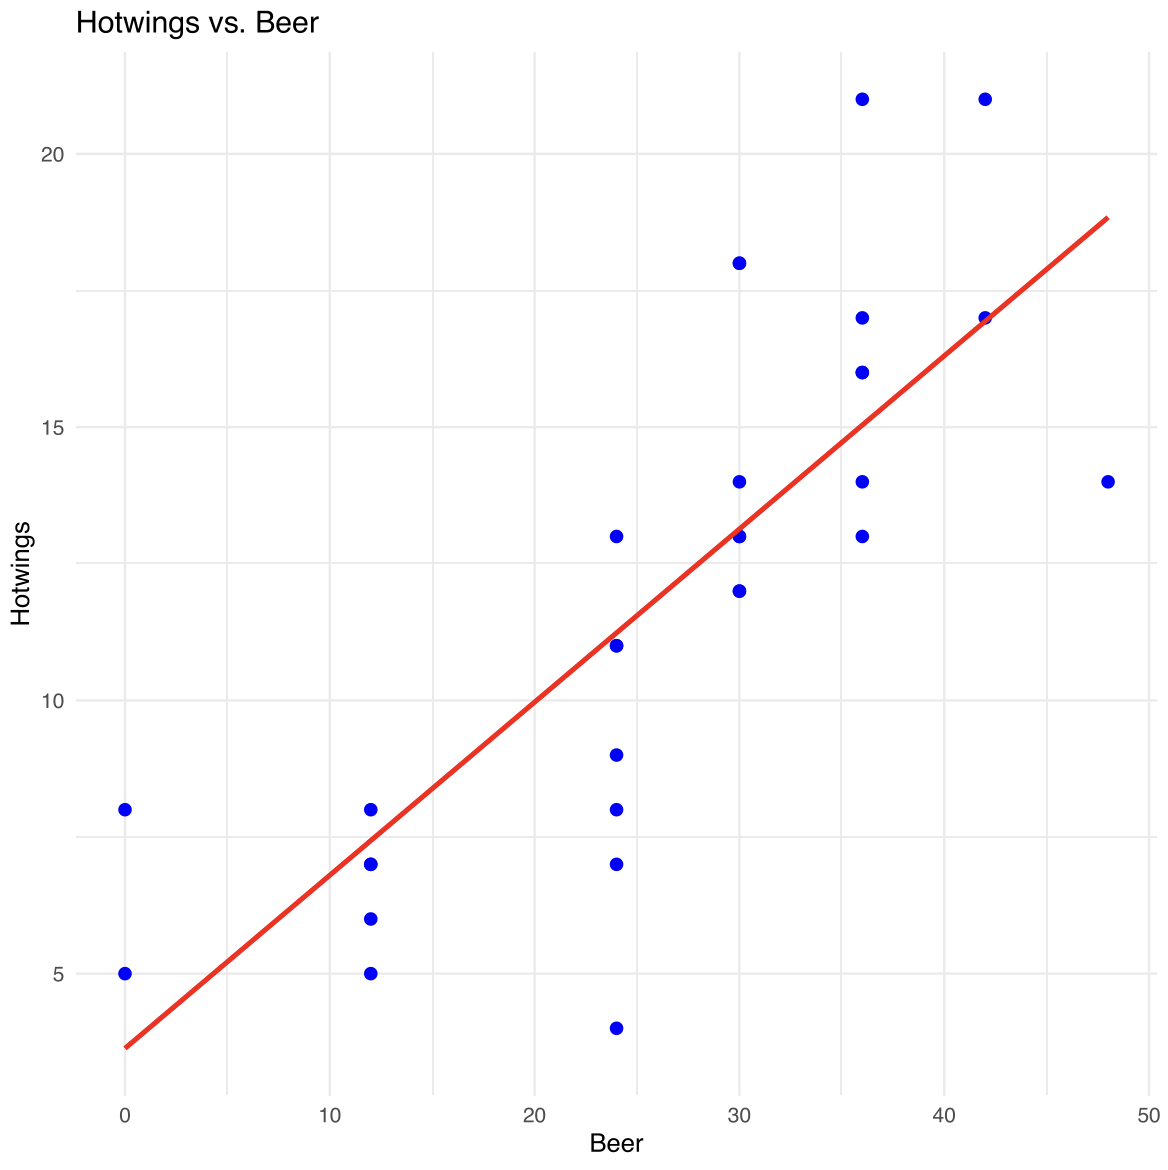
\includegraphics[width=0.5\textwidth]{hotwings_vs_beer.png}
        \end{center}
        \caption{Scatterplot of Hotwings vs. Beer}\label{fig:}
      \end{figure}
      \vspace{0.25in}
      \subsection{Fitting a Linear Model}
      We will now fit a linear model \verb|Hotwings ~ Beer|. We will use an 80-20 train-test split. 
      \vspace{0.1in} 
      \begin{lstlisting}
      fit_linear_model <- function(y, x, raw_data) {

        # train test split
        n <- nrow(raw_data)
        trainIndex <- sample(n, round(0.8 * n, 0))
        train <- raw_data[trainIndex, ]
        test <- raw_data[-trainIndex, ]
  
        # construct formula
        formula <- as.formula(paste(y, "~", x))
  
        # fit model
        model <- lm(formula, data = train)

        # Store model summary
        model_summary <- summary(model)
        print(model_summary)  # This will print the summary when the function runs
  
        # predict on testing data
        y_test <- test[[y]]
        y_hat <- predict(model, newdata = test)
  
        # analyze accuracy
        SSE <- sum((y_test - y_hat)^2)
        MSE <- SSE / nrow(test)  
        RMSE <- sqrt(MSE)
        SST <- sum((y_test - mean(y_test))^2)
        R2 <- 1 - SSE / SST
  
        return(list(
          summary = model_summary,  # Include summary in return value
          SSE = SSE, 
          MSE = MSE, 
          RMSE = RMSE, 
          SST = SST, 
          R2 = R2
        ))
      }
      \end{lstlisting}
      \vspace{0.1in}
      We will now show our linear model in the form \(\hat{y} = \beta_0 + \beta_1 x\)
      \[
        \hat{y} = 3.41405 + 0.31241x
      \]
      We find that the linear model returns a root mean squared error of RMSE = 2.8019. 
      \vspace{0.25in}
      \subsection{Scatterplot of Hotwings vs. Beer with Gender}
      We will now add a color aesthetic "Gender" to our scatterplot.
      \vspace{0.1in}
      \begin{figure}[h]
        \begin{center}
          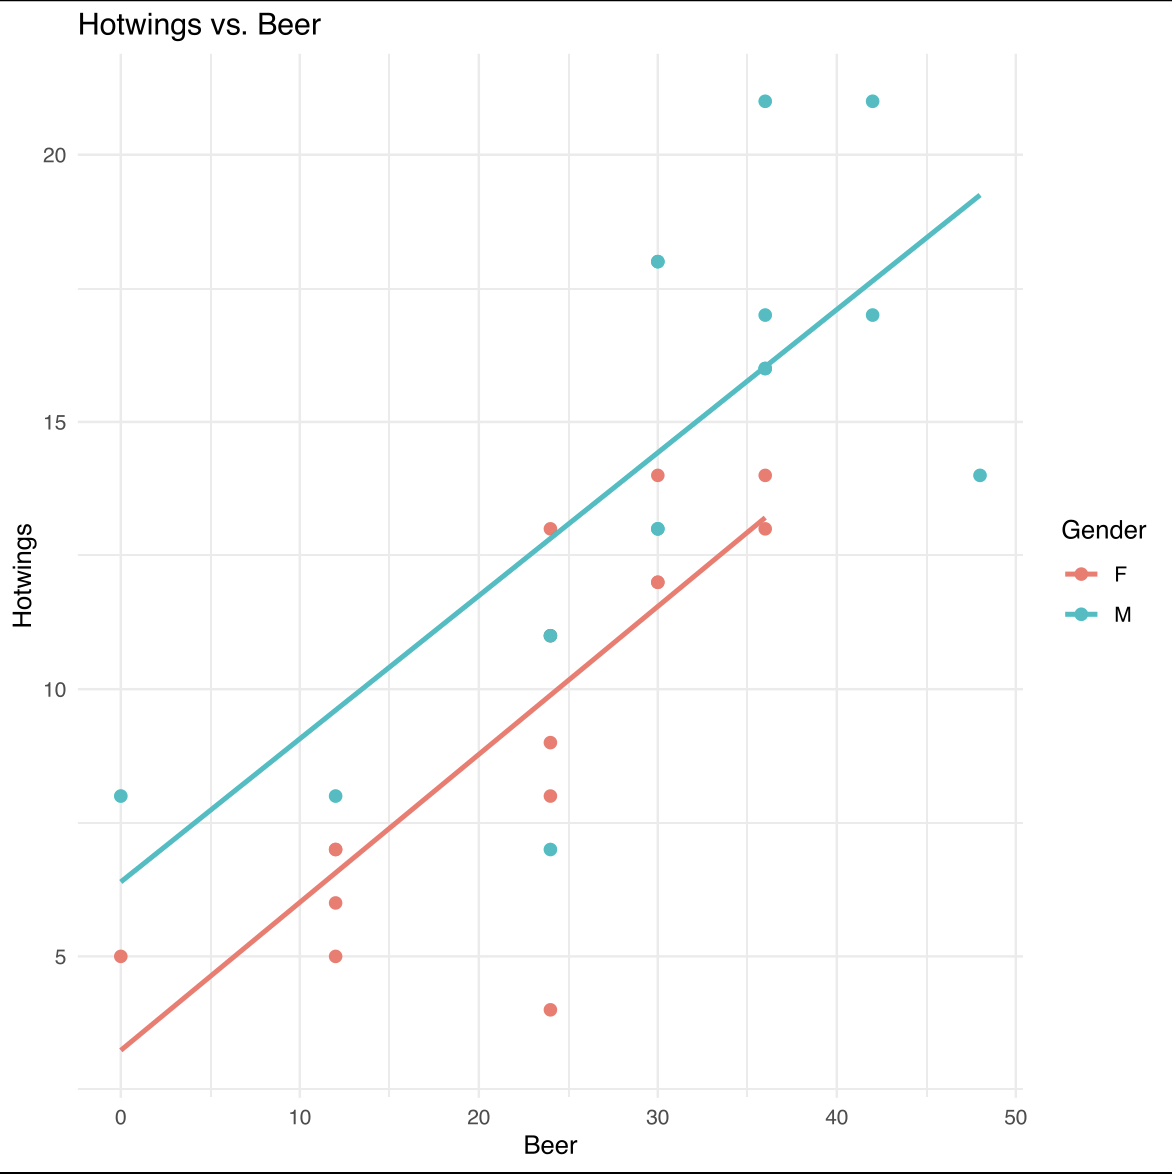
\includegraphics[width=0.5\textwidth]{hotwings_vs_beer_with_gender.png}
        \end{center}
        \caption{Scatterplot of Hotwings vs. Beer grouped by Gender}\label{fig:}
      \end{figure}
      \vspace{0.1in}
      We observe that the trendlines for men and women appear to have similar slopes, while the y-intercept for men is higher than that of women
      
\end{document}
